%\usepackage{graphicx}

\chapter{Plan}\label{ch:plan}

\section{Proposal}

Our thesis aims to provide a more personlized view of Facebook's feed that is more adaptable to users. We do this through the introduction of user types in order to figure out what users actually want in their feed. We utilize the same tried and true algorithms used in ranking the feed but we incorporate user types and the weights that are produced from this type in order to make the feed more relevant to the user. This means that users will be provided with posts that they are more interested in at the top of their feed. 

\section{User Modelling}

To determine the different user types that users of our system will be able to select from, we will perform a survey spanning a variety of different topographies as mentioned in the Background Research section. If the survey results do not yield any significant preference patterns for users, we can fallback to asking users to complete a short version of our survey upon login to our system. This way, we can still generate a list of preferences for each individual user - the only tradeoff is less convenience for the user.

\section{Overall Design of the System}

\begin{center}
  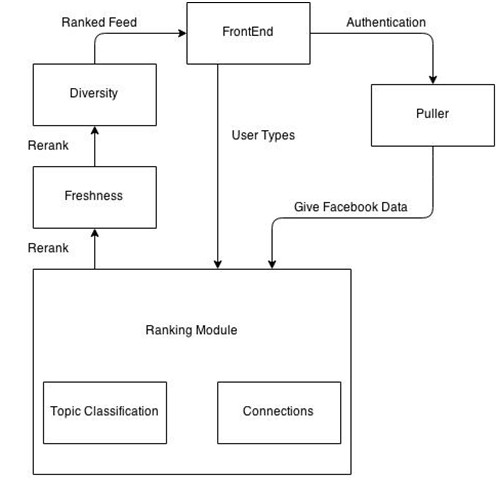
\includegraphics[scale=0.6]{images/blockdiagram.jpg}
  \captionof{figure}{Block Diagram}
\end{center}

Figure 3.1 provides a general overview of our implementation plan. It is a block diagram of our system. 

In our design, we will have a front end module which will be the website that is seen be the user. The website will have a login screen for user authentication which will allow us to pull the data from their Facebook feed. This is the job of the puller module.  The user will be given a couple of options of which user type that they think they are. The associated weights from the user types will be brought into the ranking module which contains two algorithms, one for topic classification and one for connections. The puller module will pull the feed in data into this ranking module which will rank the feed using the total scores from the topic classification, connection module and the assigned weights of the user types that came from the website or front end. To do topic classification we will look at the user's posts and try to generalise the topic based on what they have written. We will use the method proposed by Szo~\cite{szomszor2008semantic} to do topic classification.
The connections module will simply look at how often the user has interacted with the person who posted that item and give a score based on that. 

After the scores have been assigned to each post,  the feed will be ranked on the score and passed over to the freshness module. We will use Aga's~\cite{Aga2014} method and assign a decay factor to feeds that are not as recent. This feed will be reranked based on the new scores and passed over to the diversity module. In this module, we will rerank the feed and add a negative score to consecutive posts of the same type. Lastly, the newly ranked feed will be displayed in the frontend in front of the user.

We plan to use nodejs to do the whole project due to its flexibility and adaptability. We will use some written nodejs API's in order to interact with the Facebook API. 
Our timeline is shown below.

\begin{center}
  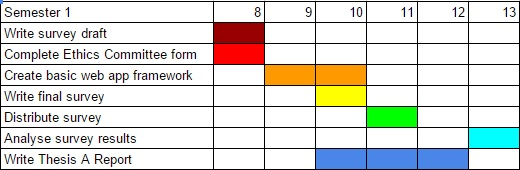
\includegraphics[scale=0.8]{images/sem1thesis.jpg}
  \captionof{figure}{Semester 1 Timeline}
\end{center}

\begin{center}
  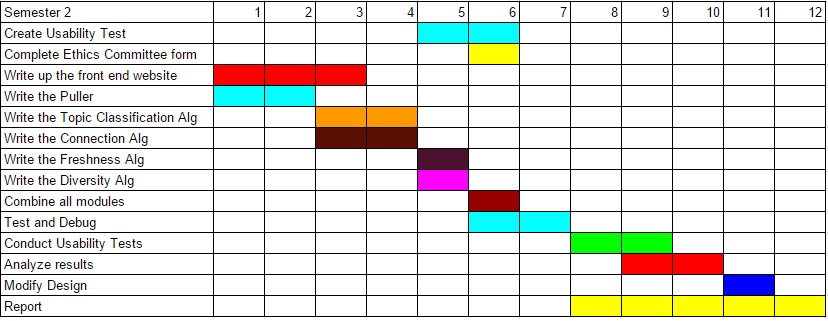
\includegraphics[scale=0.8]{images/sem2thesis.jpg}
  \captionof{figure}{Semester 2 Timeline}
\end{center}
\section {Evaluation Plan}

We considered two different ways of evaluating our system.

The first method was to simulate real users by creating Facebook accounts and attempting to mimic behaviour of each user type. We would then create a ground truth regarding how that type of user would like their feed ranked and compare the output of our ranking algorithm to the ground truth. We found quite a few flaws in this method, the major one being how difficult it would be to simulate a real user. Creating social interactions and simulating connections between users would prove very difficult. On top of this, the ground truths that we would be creating could be affected by confirmation bias. This left us with a very questionable evaluation method, so we arrived at our second one.

The second, and chosen evaluation method takes the form of gathering real users and performing a form of usability test. In this test, we will ask participants to order their feeds how they would like it to be seen, this forms an unbiased ground truth. We then run our ranking algorithm on their feeds and compare the ground truth they gave us earlier to the output. In addition to this ground truth comparison, we will ask the user to compare our ranking algorithm with the one provided by Facebook, without telling them which is which. This will give us some subjective results as to whether our ranking algorithm has succeeded in personalising the user's feed.